% ~~~ [ Control Flow Analysis ] ~~~~~~~~~~~~~~~~~~~~~~~~~~~~~~~~~~~~~~~~~~~~~~~~

\subsubsection{Control Flow Analysis}
\label{sec:lit_review_control_flow_analysis}

The control flow analysis stage is responsible for analysing the control flow (i.e. flow of execution) of source programs to recover their high-level control flow structures. The control flow of a given function is determined by its branching instructions and may be expressed as a control flow graph (CFG), which is a connected graph with a single entry node (the function entry point) and zero or more exit nodes (the function return statements). A key insight provided by C. Cifuentes and S. Moll is that high-level control flow primitives (such as 1-way conditionals and pre-test loops) may be expressed using graph representations~\cite{reverse_comp, decomp_of_llvm}, as illustrated in figure~\ref{fig:graph_representations}. The problem of recovering high-level control flow primitives from CFGs may therefore be reformulated as the problem of identifying subgraphs (i.e. the graph representation of a high-level control flow primitive) in graphs (i.e. the CFG of a function) without considering node names. This problem is commonly referred to as \textit{subgraph isomorphism search}, the general problem of which is NP-hard~\cite{subgraph_isomorphism_algorithms}. However, the problem which is required to be solved by the control flow analysis stage may be simplified by exploiting known properties of CFGs (e.g. connected graph with a single entry node).

\begin{figure}[htbp]
	\centering
	% if
	\begin{subfigure}[ht]{0.23\textwidth}
		\centering
		\begin{subfigure}[ht]{0.45\textwidth}
			\lstinputlisting[language=go, style=go, breaklines=false, numbers=none]{inc/primitives/if.c}
		\end{subfigure}
		\begin{subfigure}[ht]{0.42\textwidth}
			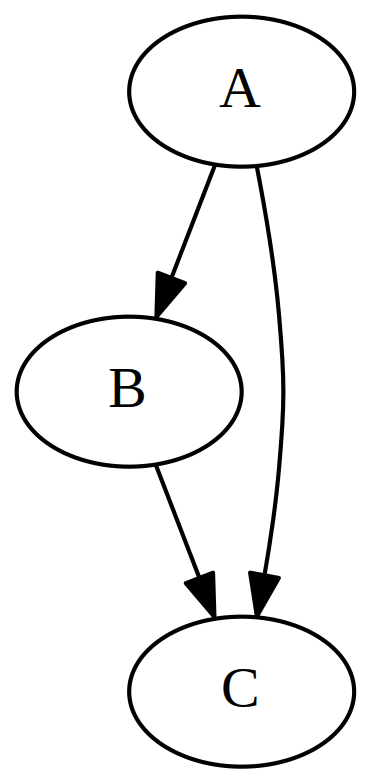
\includegraphics[width=\textwidth]{inc/primitives/if.png}
		\end{subfigure}
		\caption{1-way conditional; entry: \texttt{A}, exit: \texttt{C}.}
		\label{fig:if_graph_representation}
	\end{subfigure}
	\qquad
	% if_else
	\begin{subfigure}[ht]{0.28\textwidth}
		\centering
		\begin{subfigure}[ht]{0.45\textwidth}
			\lstinputlisting[language=go, style=go, breaklines=false, numbers=none]{inc/primitives/if_else.c}
		\end{subfigure}
		\begin{subfigure}[ht]{0.50\textwidth}
			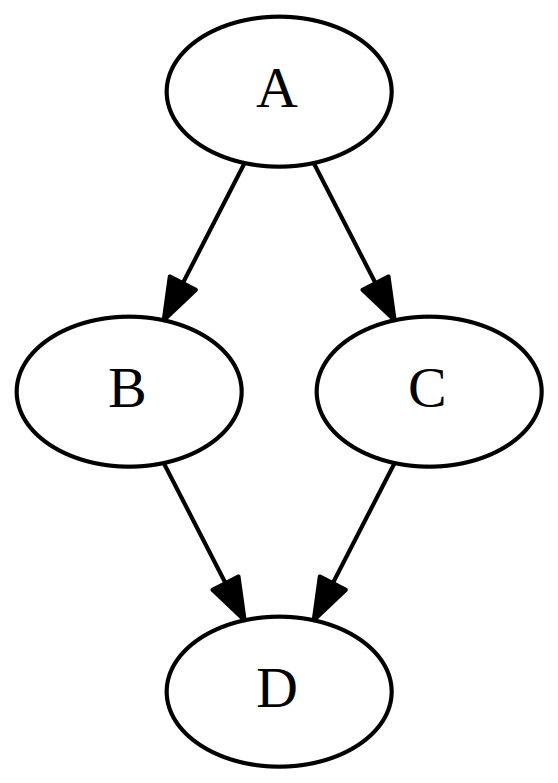
\includegraphics[width=\textwidth]{inc/primitives/if_else.png}
		\end{subfigure}
		\caption{2-way conditional; entry: \texttt{A}, exit: \texttt{D}.}
		\label{fig:if_else_graph_representation}
	\end{subfigure}
	\qquad
	% if_return
	\begin{subfigure}[ht]{0.30\textwidth}
		\centering
		\begin{subfigure}[ht]{0.45\textwidth}
			\lstinputlisting[language=go, style=go, breaklines=false, numbers=none]{inc/primitives/if_return.c}
		\end{subfigure}
		\begin{subfigure}[ht]{0.50\textwidth}
			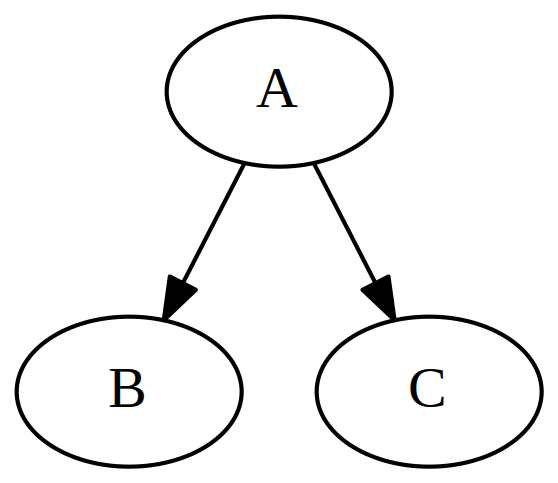
\includegraphics[width=\textwidth]{inc/primitives/if_return.png}
		\end{subfigure}
		\caption{1-way condition with return statement in body; entry: \texttt{A}, exit: \texttt{C}.}
		\label{fig:if_return_graph_representation}
	\end{subfigure}
	\qquad
	% pre_loop
	\begin{subfigure}[ht]{0.32\textwidth}
		\centering
		\begin{subfigure}[ht]{0.45\textwidth}
			\lstinputlisting[language=C, style=go, breaklines=false, numbers=none]{inc/primitives/pre_loop.c}
		\end{subfigure}
		\begin{subfigure}[ht]{0.50\textwidth}
			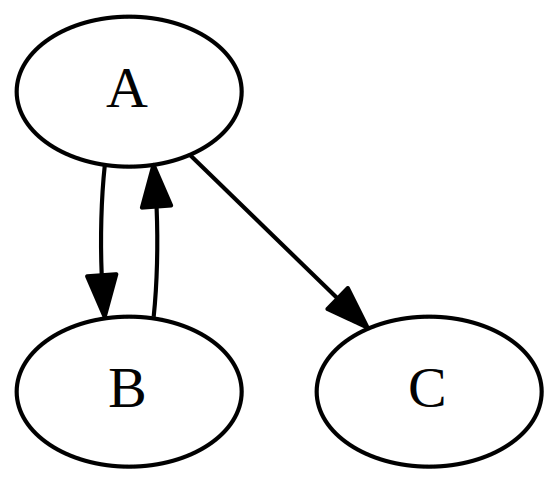
\includegraphics[width=\textwidth]{inc/primitives/pre_loop.png}
		\end{subfigure}
		\caption{pre-test loop; entry: \texttt{A}, exit: \texttt{C}.}
		\label{fig:pre_loop_graph_representation}
	\end{subfigure}
	\qquad
	% post_loop
	\begin{subfigure}[ht]{0.30\textwidth}
		\centering
		\begin{subfigure}[ht]{0.50\textwidth}
			\lstinputlisting[language=C, style=go, breaklines=false, numbers=none]{inc/primitives/post_loop.c}
		\end{subfigure}
		\begin{subfigure}[ht]{0.35\textwidth}
			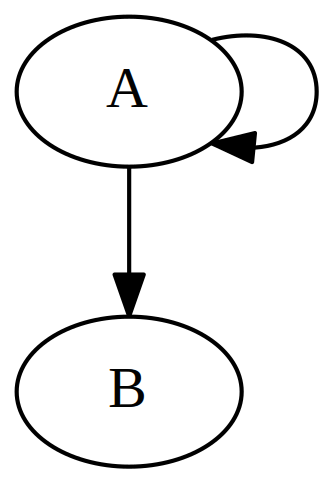
\includegraphics[width=\textwidth]{inc/primitives/post_loop.png}
		\end{subfigure}
		\caption{post-test loop; entry: \texttt{A}, exit: \texttt{B}.}
		\label{fig:post_loop_graph_representation}
	\end{subfigure}
	\qquad
	% seq
	\begin{subfigure}[ht]{0.24\textwidth}
		\centering
		\begin{subfigure}[ht]{0.20\textwidth}
			\lstinputlisting[language=C, style=go, breaklines=false, numbers=none]{inc/primitives/seq.c}
		\end{subfigure}
		\begin{subfigure}[ht]{0.35\textwidth}
			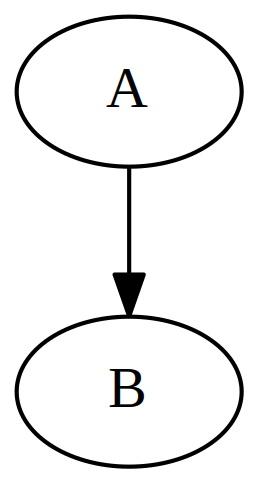
\includegraphics[width=\textwidth]{inc/primitives/seq.png}
		\end{subfigure}
		\caption{consecutive statements; entry: \texttt{A}, exit: \texttt{B}.}
		\label{fig:seq_graph_representation}
	\end{subfigure}
	\caption{The pseudo-code and graph representation of various high-level control flow primitives with denoted entry and exit nodes.}
	\label{fig:graph_representations}
\end{figure}

When the subgraph isomorphism of a high-level control flow primitive has been identified in the CFG of a function, it may be replaced by a single node that inherits the predecessors of the subgraph entry node and the successors of the subgraph exit node; as illustrated in figure~\ref{fig:subgraph_merge}. By recording the node names of the identified subgraphs and the name of their corresponding high-level control flow primitives, the high-level control flow structure of a CFG may be recovered by successively identifying subgraph isomorphisms and replacing them with single nodes until the entire CFG has been reduced into a single node; as demonstrated by the step-by-step simplification of a CFG in appendix~\ref{app:control_flow_analysis_example}. Should the control flow analysis fail to reduce a CFG into a single node, the CFG is considered irreducible with regards to the supported high-level control flow primitives (see figure~\ref{fig:graph_representations}). To structure arbitrary irreducible graphs, S. Moll applied node splitting (which translates irreducible graphs into reducible graphs by duplicating nodes) to produce functionally equivalent target programs~\cite{decomp_of_llvm}. In contrast, C. Cifuentes focused on preserving the structural semantics of the source program (which may be required in forensics investigations), and therefore used \texttt{goto}-statements in these cases to produce unstructured target programs.

\begin{figure}[htbp]
	\centering
	\begin{subfigure}[ht]{0.15\textwidth}
		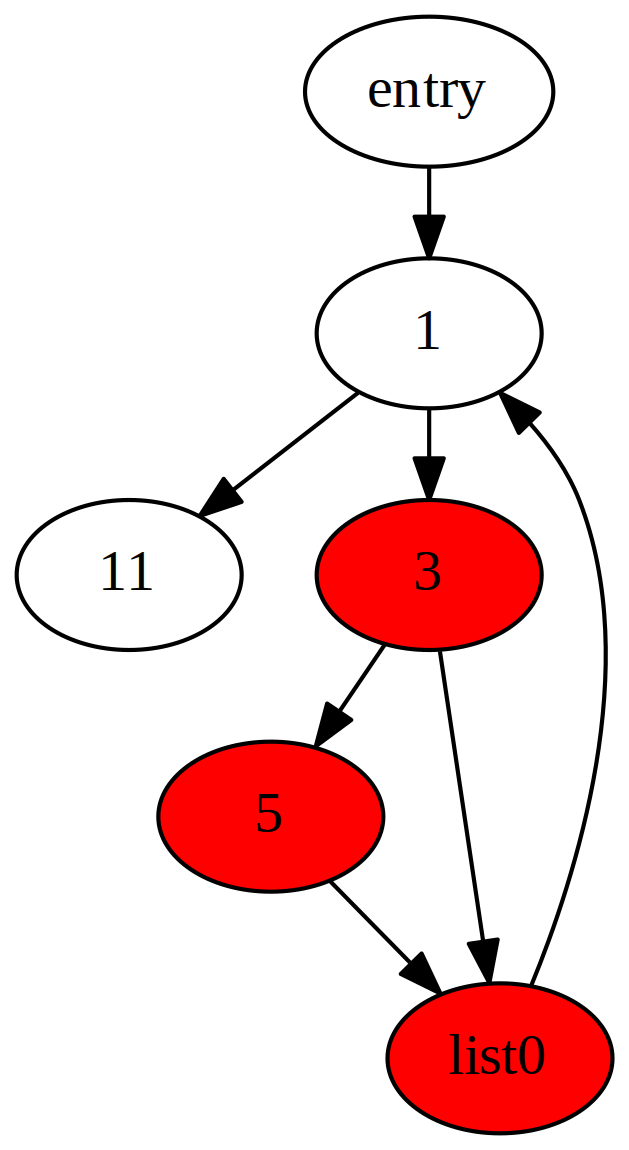
\includegraphics[width=\textwidth]{inc/2_lit_review/cfg_pre_merge.png}
	\end{subfigure}
	\qquad
	\begin{subfigure}[ht]{0.15\textwidth}
		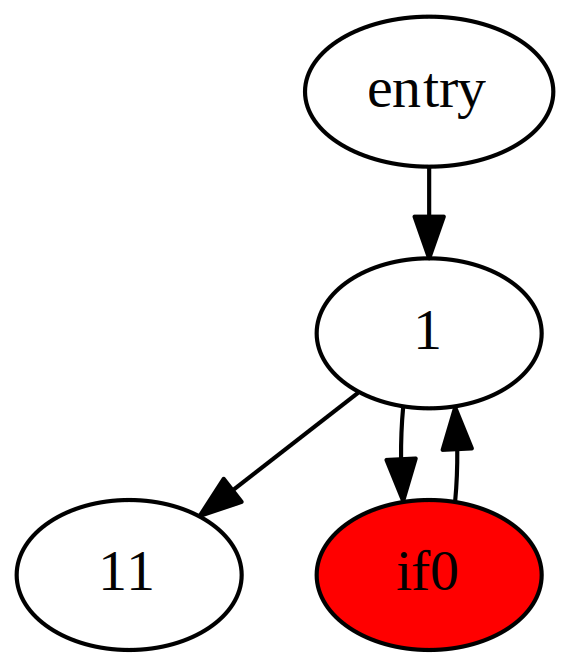
\includegraphics[width=\textwidth]{inc/2_lit_review/cfg_post_merge.png}
	\end{subfigure}
	\caption{The left side illustrates the CFG of a function in which the graph representation of a 1-way conditional (see figure~\ref{fig:if_graph_representation}) has been identified, and the right side illustrates the same CFG after the subgraph has been replaced with a single node (i.e. \texttt{if0}) that inherits the predecessors of the subgraph entry node (i.e. \texttt{3}) and the successors of the subgraph exit node (i.e. \texttt{list0}).}
	\label{fig:subgraph_merge}
\end{figure}
